\documentclass[12pt,a4paper]{article}
\usepackage{graphicx, amsmath, amssymb, indentfirst, amsfonts}
\usepackage{float} % Required for [H] placement specifier
\setlength{\parindent}{0.2in} % Indentation length setting
\setlength{\parskip}{1mm} % Paragraph spacing setting

\title{Notes on the Kalman Filter}
\author{Sehwan Jhang}
\date{September 2024}
\begin{document}
\maketitle

\section{Preliminaries}
The Kalman filter is an algorithm that recursively predicts and
updates the state of a time-varying system based on predictions from the system model
and noisy observations.
This section provides a brief overview of the foundational knowledge before delving
into the Kalman filter itself.

\subsection{Estimation Theory}

Estimation theory encompasses various methods for predicting the parameters
of a model based on observed data. It is widely used in fields such as data analysis,
machine learning, finance, and robotics, serving as an essential tool for making accurate predictions
in the presence of uncertainty.

\begin{figure}[!htbp] % Force placement
    \centerline{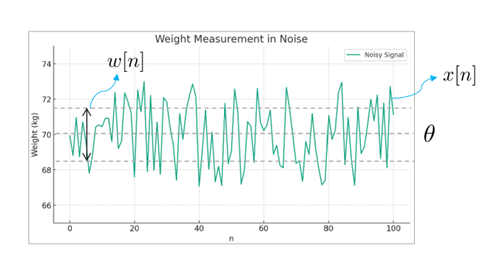
\includegraphics[width=10cm]{image1.png}}
    \caption{Example of data used in estimation theory.}
\end{figure}

For example, suppose we are given data measured over a year for a person whose average
weight is 70 kg, as shown in the figure above.
The green data points forming the graph are \(x[n]\), and the central value of these data points is the parameter \(\theta\) that we aim to estimate.
The degree of spread (i.e., variance) around \(\theta\) can be mathematically represented by \(w[n]\).
The problem of estimating the parameter \(\theta\) based on the observed data \(x[n]\) can be expressed
by the following simple mathematical model:
\begin{equation}
    x[n] = \theta + w[n]= 0, 1, \ldots, N - 1
\end{equation}
\begin{itemize}
    \item \(x[n]\) : observed data,
    \item \(\theta\) : parameter to be estimated,
    \item \(w[n]\) : random noise.
\end{itemize}

\subsection{Bayesian Philosophy}

Estimation theory can be broadly divided into two perspectives: the frequentist and the Bayesian, depending
on how the parameter \(\theta\) to be estimated is viewed.

\begin{itemize}
    \item Frequentist : A frequentist perspective views the parameter \(\theta\) as an unkown deterministic parameter.
    \item Bayesian : A Bayesian perspective treats the paramter \(\theta\) as a random variable with a prior probability distribution.
\end{itemize}

\begin{equation}
    \begin{aligned}
        \text{Frequentist:} \quad & \underbrace{x[n]}_{\text{r.v.}} = \underbrace{\theta}_{\text{deterministic}} + \underbrace{w[n]}_{\text{r.v.}} \\
        \text{Bayesian:} \quad    & \underbrace{x[n]}_{\text{r.v.}} = \underbrace{\theta}_{\text{r.v.}} + \underbrace{w[n]}_{\text{r.v.}}
    \end{aligned}
\end{equation}

The Bayesian philosophy starts from the premise theat if we have prior information about the
paramteter \(\theta\), it can be used to make a better estimate. For this, a prior pdf of \(\theta\) must be provided
or computable.
In the Bayesian framework, since the parameter \(\theta\) can also be modeled as a random variable,
the following Bayesian rule holds:
\begin{equation}
    p(\theta \mid x) = \frac{p(\theta)p(x \mid \theta)}{p(x)}
\end{equation}
\begin{itemize}
    \item  p(\(\theta\mid x\)) : posterior conditional probability distribution of the parameter \(\theta\) given the observed data \(x\)
    \item p(\(x\mid \theta\)) : conditional probability distribution of \(x\) given \(theta\), or likelihood
    \item p(\(x\)) : probability distribution of x
    \item p(\(\theta\)) : prior probability distribution of \(theta\)
\end{itemize}

\subsection{Estimation problem}

\begin{figure}[H] % Place the figure exactly here
    \centering
    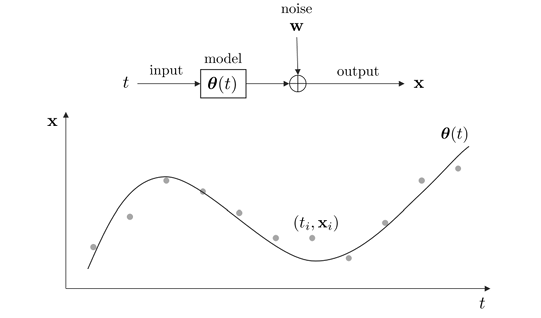
\includegraphics[height=6cm,width=10cm]{image2.png}
    \caption{Example of data used in estimation theory.}
\end{figure}

The goal of the estimation problem is to find the optimal model \(\theta(t)\) using the given data \((t_{i}, x_{i})\). The type of estimation problem varies depending on which point in time is being estimated.

\begin{figure}[H] % Place the figure exactly here
    \centering
    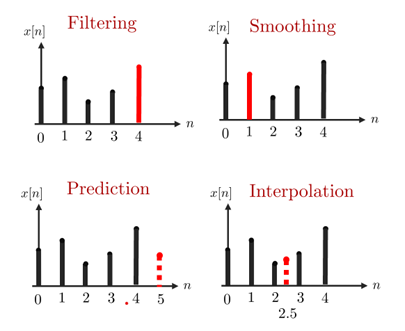
\includegraphics[height=5cm,width=10cm]{image3.png}
    \caption{Example of data used in estimation theory.}
\end{figure}

\begin{enumerate}
    \item \textbf{Filtering}: Filtering refers to the problem of estimating \(\theta = x[N - 1]\) given the observed data \(\{x[0], x[1], \dots, x[N - 1]\}\). By estimating the optimal parameter, we aim to filter out the noise from the signal. Note that in filtering, the parameter depends only on current and past data.

    \item \textbf{Smoothing}: Smoothing refers to the problem of estimating an intermediate \(\theta = s[n]\) given the observed data \(\{x[0], x[1], \dots, x[N - 1]\}\). For instance, to estimate \(s[1]\), all observed data are used. Naturally, smoothing cannot be performed until all data are observed.
    \item \textbf{Prediction}: Prediction refers to the problme of estimating \(\theta  = x[N - 1 + l]\) given the
          observed data \(\{x[0], x[1], \dots, x[N - 1]\}\). Here, \(l\) is an arbitrary positive number.

\end{enumerate}


\end{document}
